\documentclass[10pt,authoryear,a4paper,review]{elsarticle}
\usepackage[utf8]{inputenc}

\usepackage{geometry}
\newgeometry{margin=2.5cm}

\journal{Computers and Electronics in Agriculture}

\usepackage{amsmath}
\usepackage{hyperref}

\usepackage{cleveref}

\usepackage{siunitx}

\usepackage{tabularx}
\usepackage{booktabs}
\usepackage{colortbl}
\usepackage{xcolor}

\usepackage{xparse}
\NewDocumentCommand{\dutch}{m}{Dutch: \textit{#1}}

%\usepackage{lineno}

\begin{document}

\begin{frontmatter}

    \title{Limitations of snapshot hyperspectral cameras to monitor plant response dynamics in stress-free conditions}
    
    \author[a,b]{Olivier~Pieters}
    \ead{olivier.pieters@ugent.be}
    \ead[url]{olivierpieters.be}
    
    \author[b]{Tom~De~Swaef}
    \ead{tds@ilvo.be}
    
    \address[a]{Ugent, Zwijnaarde}
    \address[b]{ILVO, Melle}
    
    \begin{abstract}
        In perennial ryegrass breeding programs, dry matter yield (DMY) of
        individual plots is monitored destructively at the different cuts or
        derived from non-destructive canopy height measurements using devices
        like rising plate meters (RPM). These approaches both have constraints.
        Destructive sampling implies low temporal resolution, restraining the
        study of dry matter accumulation rates, while RPM measurements are
        influenced by the canopy structure and limit intra-field variability
        identification. We present a phenotyping methodology, based on the use
        of an affordable RGB camera mounted on an Unmanned Aerial Vehicle (UAV),
        to monitor the spatial and temporal evolution of canopy height and to
        estimate DMY. Weekly flights were carried out from April to October
        above a field comprising a diverse set of accessions. To test the
        capability of the model extracted from the data to estimate canopy height, 
        8~ground control points and 28~artificial height references were placed 
        at different locations. Accurate flights with an RMSE as low as 0.94~cm were
        achieved. In addition, canopy height was recorded using an RPM and
        destructive biomass samples were collected. Different models (linear,
        multiple linear, principal components, partial least squares regression
        and random forest) were used to predict DMY and their performance was
        evaluated. The best estimations were obtained by combining variables
        including canopy height, vegetation indices and environmental data in a
        multiple linear regression (${R^2 = 0.81}$). All models built using UAV data
        obtained a lower RMSE than the one using RPM data. The approach
        presented is a possibility for breeders to incorporate new information
        in their selection process.
    \end{abstract}
    
    \begin{highlights}
        \item Study of very important sensors
        \item It did not work as hypothesised
    \end{highlights}
    
    \begin{keyword}
        Hyperspectral camera\sep phenotyping\sep monitoring
    \end{keyword}

\end{frontmatter}

%\linenumbers

\section{Introduction}
 
    Plants adapt their physiology continuously in response to fluctuations in the environment. This determines their performance, both in natural ecosystems, as well as in crop systems \citep{schurrFunctional2006,arsovaDynamics2020}. An increasing amount of experimental data suggests that proper acclimation of the photosynthesis biochemistry to environmental fluctuations is crucial for plant productivity, and potentially more important than high photosynthesis rates under steady-state conditions \citep{kaiserFluctuating2018,kromdijkImproving2016,vialet-chabrandImportance2017,matthewsAcclimation2018,townsendSuboptimal2018}.
    For instance, when focussing on the water relationships in a plant, changes in the environment cause variation in stomatal conductance which in turn determines leaf transpiration, and consequently leaf cooling as well as plant nutrient uptake.
 
    For example, because the response of the photosynthesis biochemistry to fluctuating light conditions is faster than the kinetics of stomatal conductance, these fluctuations also impact the interplay between plant water and carbon relations \citep{lawsonImproving2012,lawsonStomatal2014}. Consequently, a mismatch arises between CO\textsubscript{2} assimilation and water loss \citep{mcauslandEffects2016}. Reducing this mismatch, and improving the capacity of crop photosynthesis to respond to fluctuating light environments is, therefore, a promising avenue for breeding more productive crop varieties \citep{salterRate2019,murchieDynamic2020}. 
 
    Given the importance of plant physiological responses to environmental fluctuations,  it is essential that new field phenotyping technologies specifically focus on capturing such fast-changing dynamics \citep{murchieMeasuring2018}. Yet, it remains difficult to capture plant photosynthetic and water status responses to fluctuating conditions in the field. Gas exchange devices based on infrared gas analysers (IRGA) allow continuous measurements of transpiration and CO\textsubscript{2} assimilation and capture detailed dynamics \citep{kromdijkImproving2016}. However, this approach does not allow for high-throughput measurements and requires expensive devices. Furthermore, these systems monitor individual leaves and do not provide concurrent data at the plant scale, while recent evidence points out that plants display systemic responses under fluctuating light conditions \citep{shimadzuWhole2019}. 
 
    Chlorophyll fluorescence imaging is a powerful method to monitor the photosynthetic capacity of plants \citep{bakerChlorophyll2008,murchieChlorophyll2013}. However, chlorophyll fluorescence measurements typically require a dark adaptation period of one hour, which limits the applicability to study short-term dynamics. New developments in chlorophyll fluorescence imaging methods like Light-Induced Fluorescence Transient (LIFT) or Sun Induced Fluorescence (SIF) overcome this dark adaptation period and can be used as proxies. These methods can be applied at different scales and show great promise, though they do not enable acquisition of absolute photosynthesis biochemistry data, and still require extensive calibration \citep{murchieDynamic2020,bandopadhyayReview2020}.
 
    Moreover, chlorophyll fluorescence imaging is unable to monitor stomatal conductance. Because stomatal conductance is closely related to leaf temperature, thermal sensors can be used to monitor it by applying basic energy balance equations \citep{jonesIrrigation2004,maesEstimating2012}. These equations require the assessment of the micro-environmental conditions of the leaf and the boundary layer resistance to water vapour \citep{jonesUse2002}. Although most studies with thermal sensors use single time point observations, continuous monitoring of dynamic stomatal conductance in response to a fluctuating environment is possible and can be combined with chlorophyll fluorescence imaging to link plant water relations and photosynthesis \citep{mcauslandEffects2016}. 
 
    Generally, field phenotyping uses imagery that captures the plants' reflectance in different wavelengths. This information can be used to determine specific plant traits. Examples include, but are not limited to, detection of biotic and abiotic stress, and estimation of nitrogen content and yield. \citet{mirHighthroughput2019} provides an overview of current methods. In this respect, broadband RGB cameras are often used in phenotyping experiments because they are inexpensive and can be used to monitor plant growth at the scale of days and weeks, or to develop spectral indices referring to the greenness or canopy cover \citep{borra-serranoClosing2020}. However, these sensors do not provide information on dynamic responses of photosynthesis over time scales of seconds or minutes.
 
    Hyperspectral imaging sensors capture reflectance in many wavelengths and are increasingly applied in phenotyping research. Hyperspectral imaging has already been applied to various settings that benefit from higher spectral resolutions to detect biotic and abiotic influences on plants \citep{khanModern2018}. Examples of studies on biotic factors include blight caused by \textit{Alternaria solani} in potato \citep{vandevijverInfield2020}, late blight caused by \textit{Phytophthora infestans} in potato \citep{franceschiniFeasibility2019}, or tracking the development of three foliar diseases in barley \citep{wahabzadaPlant2016}. \citet{mahleinPlant2015} and \citet{loweHyperspectral2017} provide comprehensive overviews of plant disease detection using imaging sensors and hyperspectral sensors specifically. Studies in which hyperspectral imaging was used to investigate plant responses in interaction with abiotic factors include, for example, detection of green citrus fruits on trees \citep{okamotoGreen2009}, nitrogen deficiency in sorghum, seasonal structural changes and a heterogeneous architecture in an olive orchard \citep{zarco-tejadaSpatiotemporal2013}, nitrogen and water distribution quantification in wheat \citep{bruningDevelopment2019}, and drought stress in barley and saxaul \citep{behmannDetection2014,jinHyperspectral2016}. One common aspect that all the aforementioned studies share, is the presence of a clear treatment or perturbation that results in substantial stress or that influences the phenology of the plant. Furthermore, they usually monitor plants over extended periods, often months or an entire growing season, typically with several days to a week between measurements. 
 
    However, to the best of our knowledge, there is no research yet on hyperspectral data concerning photosynthetic activity at high spatial and temporal resolution in the seconds to minutes range. Nonetheless, vegetation indices (VI) and data derived from hyperspectral cameras might have the potential to monitor subtle dynamics on a detailed scale. For instance, the Photochemical Reflectance Index (PRI) offers potential if it can capture variations in the de-epoxidation of the xanthophyll cycle \citep{alonsoDiurnal2017} or the Canopy Chlorophyll Content Index (CCCI) which offers a good measure of canopy nitrogen \citep{barnesCoincident2000}. 
 
    We believe that new phenotyping technologies should increasingly focus on capturing dynamics in photosynthesis biochemistry and stomatal conductance kinetics under stress-free yet fluctuating conditions. The objective of the present study is to evaluate the potential of hyperspectral snapshot cameras for this purpose. More specifically, we aim to capture the dynamic responses of strawberry plants in fluctuating, yet stress-free environmental conditions. To this end, experiments were conducted in growth chambers because they offer excellent controllability of the environment over field experiments.

\section{Materials and Methods}
    
    The experimental set-up consisted of a single strawberry plant (Fragaria $\times$ ananassa), placed inside a growth chamber of \SI{1.45 x 0.77 x 1.45}{\metre} (height $\times$ depth $\times$ width) (BIOCLIM 1600 US, Weiss Technik, Reiskirchen, Germany). Light intensity, temperature and relative humidity were controlled by a micro-controller board (Dwenguino, Dwengo vzw, Brussels, Belgium), placed outside the growth chamber. The temperature and relative humidity of the growth chamber were controlled using analogue signals, and varied randomly between \SI{11}{\celsius} and $33^{\circ}\text{C}$, and \SI{31}{\percent} and \SI{75}{\%} respectively. 
    
    A custom-built frame of \SI{1.00 x 0.70 x 1.10}{m} (height $\times$ depth $\times$ width) was inserted into the chamber. On top of which a grid of lamps was mounted, consisting of 32~LED lamps (MAS LED spot VLE D 4.9-50W GU10 927 60D, Koninklijke Philips N.V., Amsterdam, The Netherlands) and twelve halogen lights (DECOSTAR 51 PRO 50 W 12 V 36 GU5.3, OSRAM GmbH, Munich, Germany). The halogen lights were used as broadband light source, providing illumination in the visible and infrared range, while the LED lights increased the total Photosynthetically Active Radiation (PAR) while keeping thermal radiation within limits. The light intensity of the halogen lamps was controlled using a Digital Addressable Lighting Interface (DALI) controller and bus, while the LED lights were arranged in four sets that could be individually turned on and off. A detailed overview of the grid is depicted in \cref{fig:lamp-layout}. 
    
    A single strawberry leaf was inserted into a transparent leaf chamber of the LI-6400XT photosyn-thesis system (LI-COR, Lincoln, NE, USA) to acquire gas exchange measurements (transpiration and photosynthesis). The control board also controlled the sampling time steps of the LI-6400XT, using a custom circuit that was connected to the manual sample button on the measurement node. To increase the carbon dioxide concentration in the growth chamber, a constant influx of stabilised air was used. This influx had a carbon dioxide concentration of \SI{500}{ppm} at a rate of \SI{1}{\cubic\metre\per\hour}. For environment sensing at canopy height, we measured the temperature, light intensity and relative humidity. An external probe (Vaisala 50Y, Vaisala, Helsinki, Finland) was used to measure temperature and humidity. The gas ex-change device has a PAR probe to measure light intensity. This device was programmed to recreate the temperature measured using the probe inside the chamber, thus preventing the chamber from heating-up due to infrared radiation. 
    
    \begin{figure}[tb]
        \centering
        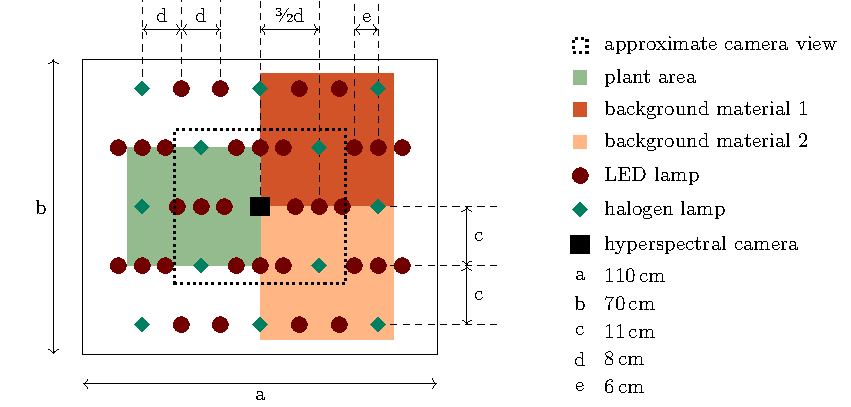
\includegraphics[width=\linewidth]{figures/lamp-layout}
        \caption{Schematic representation of the light and camera arrangement above the plant and background materials.}
        \label{fig:lamp-layout}
    \end{figure}
    
    \subsection{Data Preparation and Processing}
    
        VIs are often used to extract meaningful information from image data, also in hyperspectral imaging \citep{vogelmannRed1993}. However, only a limited and non-uniformly spaced number of bands are available here, limiting the possibilities to use VIs from literature. Therefore, we generated a custom set of VIs. Based on literature, and taking practical limitations of the number of variables into account, we limited the created VIs to combinations of fractions of band pairs, summarised by \cref{fraction1,fraction2}. All possible combinations of two spectral bands were generated. \Cref{fraction1} is the fraction (F), and \cref{fraction2} is the normalised fraction (NF) of a pair of bands. The model automatically selected the relevant indices thanks to regularisation (see below). The spectral bands from H1 were numbered 0 through 24, and those of H2 25 to 40. An index was only included if the absolute value of the maximum value of all Pearson correlation coefficients ($\rho$) with already included indices was lower than 0.95. This boundary ensures that none of the features were (nearly) linearly dependent. Note that the included VIs need not be the same for the different data types since the correlation metric might differ. This technique could generate up to 2459 new features.
        
        
        \begin{equation}
            VI_{ij}^{F} = \dfrac{C_{i}}{C_{j}}, \quad i \in \{0,1,\ldots, 40\}, j \in \{ 0,1,\ldots,i-1,i+1,\ldots,40\} 
            \label{fraction1}
        \end{equation}
        \begin{equation}
            VI_{ij}^{F} = \dfrac{C_{i} - C_{j}}{C_{i} + C_{j}}, \quad i \in \{0,1,\ldots, 39\}, j \in \{ i+1,i+2,\ldots,40\} 
            \label{fraction2}
        \end{equation}
        
        
        Normally, VIs are only generated on image data from plants, but we also generated them for the background materials to avoid bias due to the generation of possibly more informative features in the comparison between plant- and background-based models. 


    \subsection{Variables and Eco-physiological Meaning}

        The gas exchange measurement device (LI6400XT) produced the eco-physiological data to which 
        the hyperspectral image data was fitted. Different environmental and eco-physiological parameters were captured, providing a diverse set of target variables. An overview of the available variables is provided in \cref{variable-table}. All variables except for air temperature (T air ) and relative humidity (RH) were measured outside the area observed with the camera. This was a requirement due to the high reflectivity of the leaf chamber that resulted in an undesired exposure compensation of the camera. 
        
        % \usepackage{tabularx}
        % \usepackage{colortbl}
        % \usepackage{xcolor}
        \begin{table}[ht]
            \centering
            \caption{Overview of considered environmental and eco-physiological variables}
            \label{variable-table}
            \begin{tabularx}{\linewidth}{cXcc}
                \toprule
                \textbf{abbreviation} & \textbf{description} & \textbf{unit} & \textbf{sensor} \\
                \midrule
                \arrayrulecolor{black!10!white}
                $P_n$ & photosynthetic rate & \si{\micro\mole \per\metre\squared \per\second} & LI6400XT \\
                \midrule
                $VPD_\text{leaf}$ & vapour pressure deficit based on leaf temperature temperature temperature temperature temperature & \si{\milli\mole \per\square\metre \per\second} & LI6400XT \\
                \arrayrulecolor{black}
                \bottomrule
            \end{tabularx}
        \end{table}
    
        
    \bibliographystyle{elsarticle-harv}
    \bibliography{bibliography}

\end{document}
